% Exercises from Xu Chen and Masayoshi Tomizuka, "Introduction to Modern Controls
% with Illustrations in MATLAB and Python," 2023.
%
% Problem a.b is exercise b of chapter a. ctrl.js reads this file for the daily problem.
% \problem{number}{group}: problems sharing a group split one share of the daily draw,
% an empty group means the problem stands alone.
\documentclass{article}
\usepackage{amsmath,amssymb,graphicx}
\usepackage[margin=1in]{geometry}
\renewcommand{\labelenumi}{\alph{enumi})}
\newcommand{\problem}[2]{\subsection*{#1}}
\title{Control Systems Problems}
\author{From Chen and Tomizuka, \emph{Introduction to Modern Controls}}
\date{}
\begin{document}
\maketitle

\section*{2 Modeling}

\problem{2.1}{modeling-concepts}
What is the difference between a causal system and an acausal system?

\problem{2.2}{modeling-concepts}
Can a static system be acausal?

\problem{2.3}{modeling-concepts}
Can a linear system be time-varying?

\problem{2.4}{}
Solve the following ODEs:
\begin{enumerate}
\item $\ddot{y} + \dot{y} - 2y = 0$, $y(0) = 4$, $\dot{y}(0) = -5$,
\item $\ddot{y} + \dot{y} + 0.25y = 0$, $y(0) = 3$, $\dot{y}(0) = -3.5$,
\item $\ddot{y} + 0.4\dot{y} + 9.04y = 0$.
\end{enumerate}

\problem{2.5}{modeling-literature}
A quadcopter is a type of unmanned aerial vehicle (UAV) that is controlled by adjusting the speed of its four rotors. Read relevant literature and develop a mathematical model of a quadcopter.

\problem{2.6}{modeling-literature}
A robotic arm is used to move objects in a manufacturing facility. The arm consists of several joints that can be controlled to move the end-effector to a desired position. Read relevant literature. Develop a dynamic model between the torque input to the motors and the joint angles.

\problem{2.7}{modeling-literature}
A power system consists of generators, transformers, transmission lines, and loads. Read relevant literature and develop a simplified model of a power system.

\problem{2.8}{modeling-literature}
A cruise control system in a car maintains a constant speed by adjusting the throttle. The system must be able to handle changes in terrain and driving conditions. Read relevant literature and develop a simplified model of a cruise control system.

\problem{2.9}{modeling-literature}
A temperature control system in a chemical plant consists of a heater, a temperature sensor, and a controller. The controller receives input from the temperature sensor and sends a signal to the heater to adjust the temperature. Develop a block diagram of the control system and a mathematical model of the plant.

\section*{3 Laplace and Z Transforms}

\problem{3.1}{}
Consider the following two by two matrix:
\[
A = \begin{bmatrix} -5 & 2 \\ 2 & -2 \end{bmatrix}.
\]
\begin{enumerate}
\item Obtain the eigenvalues and eigenvectors of the matrix.
\item Obtain the rank of the matrix analytically, and confirm your solution by using MATLAB or Python.
\end{enumerate}

\problem{3.2}{}
Obtain the inverses of the following matrices
\[
M = \begin{bmatrix} s & -1 \\ \frac{k}{m} & s + \frac{b}{m} \end{bmatrix}, \quad
N = \begin{bmatrix} s & 6 & 0 \\ 2 & s - 1 & 0 \\ 0 & 0 & s + 1 \end{bmatrix}.
\]

\problem{3.3}{laplace-drills}
Find the Laplace transform of the function $f(t) = 2te^{-3t}$.

\problem{3.4}{laplace-drills}
Find the inverse Laplace transform of the function $F(s) = (s + 3)/(s^2 + 4s + 5)$.

\problem{3.5}{laplace-drills}
Find the Laplace transform of the function $f(t) = \sin(2t)u(t)$.

\problem{3.6}{laplace-drills}
Find the Laplace transform of the function $f(t) = te^{-2t}\cos(3t)$.

\problem{3.7}{laplace-drills}
Find the Laplace transform of the function $f(t) = t^2$.

\problem{3.8}{z-drills}
Find the Z-transform of the function $f(k) = 2^k u(k)$.

\problem{3.9}{z-drills}
Find the inverse Z-transform of the function $F(z) = (z + 2)/(z^2 - 2z + 3)$.

\problem{3.10}{z-drills}
Find the Z-transform of the function $f(k) = k^2 (0.5)^k$.

\problem{3.11}{z-drills}
Find the Z-transform of the function $f(k) = \cos(0.2\pi)u(k)$.

\problem{3.12}{z-drills}
Find the inverse Z-transform of the function $F(z) = (z^2 - z + 1)/(z - 1)^3$.

\problem{3.13}{}
Let $\mathcal{L}\{f(t)\} = F(s)$. Show that
\[
\mathcal{L}\left\{f^{(n-1)}(t)\right\} = s^{n-1}F(s) -
\begin{bmatrix} s^{n-2} & s^{n-3} & \dots & 1 \end{bmatrix}
\begin{bmatrix} f(0) \\ \dot{f}(0) \\ \vdots \\ f^{(n-2)}(0) \end{bmatrix}.
\]

\problem{3.14}{ode-drills}
Solve the ordinary differential equation $\dot{x} + 3x = 1(t)$ where $x(0) = 0$.

\problem{3.15}{}
Show that if $G(s)$ is strictly proper, then $G(\infty) = 0$.

\problem{3.16}{}
Obtain the time-domain expression of the following Laplace- and Z-domain functions:
\[
\frac{1}{(s + a)^2}, \quad \frac{Tz^{-1}}{(a - z^{-1})^2}.
\]

\problem{3.17}{laplace-drills}
Obtain $f(t)$ if $F(s) = (s + 10)/(s^2 + 2s + 5)$.

\problem{3.18}{}
Show that for systems with relative degree greater than or equal to zero, the impulse response always converges to 0.

\problem{3.19}{ode-drills}
Solve the ordinary differential equation $\ddot{x} + a_1\dot{x} + a_2 x = 0$ where $a_1 = 2$ and $a_2 = 1$.

\problem{3.20}{}
Obtain the Laplace or Z transforms of the following time functions.
\begin{enumerate}
\item Continuous-time periodic function: $f(t) = f(t - T)$, assuming $\{f(\tau) \mid 0 \le \tau < T\}$ is given.
\item Discrete-time periodic function: $f(k) = f(k - N)$, assuming $\{f(j) \mid 0 \le j < N - 1\}$ is given.
\end{enumerate}

\problem{3.21}{}
The Laplace transform of $f(t)$ is expressed as
\[
F(s) = \frac{(K_1 - K_2\tau)s + (K_1 - K_2)}{s(\tau s + 1)(s + 1)}.
\]
Assume $\tau > 0$ in this problem (think about what happens if this is not satisfied).
\begin{enumerate}
\item Use the initial value and final value theorems to obtain the conditions so that $f(t)$ possesses a negative initial slope (derivative) and a positive final value.
\item Note that $f(t)$ is regarded as the unit step response of the system described by
\[
G(s) = \frac{(K_1 - K_2\tau)s + (K_1 - K_2)}{(\tau s + 1)(s + 1)}.
\]
Assume the following values of the system parameters:
\[
K_1 = 2, \quad K_2 = 1, \quad \tau = 4.
\]
Obtain the time plot for $f(t)$ by MATLAB or Python or Julia.
\end{enumerate}

\problem{3.22}{}
Given a Z transform
\[
X(z) = \frac{z^{-1}}{(1 - z^{-1})(1 - 1.4z^{-1} + 0.48z^{-2})},
\]
determine the initial and final values of $x(k)$, the inverse Z-transform of $X(z)$. Find $x(k)$ in a closed form.

\problem{3.23}{}
Let $f(t)$ be a function that has convergent Laplace transform and $f(0^+) \neq f(0^-)$, i.e., $f(t)$ has a first-kind discontinuity at $t = 0$. Based on the definition $F(s) = \int_{0^-}^{\infty} f(t)e^{-st}dt$,
\begin{enumerate}
\item show that $\lim_{s \to \infty} sF(s) = f(0^+) \neq f(0^-)$
\item which one is true: $\mathcal{L}\left\{\frac{d}{dt}f(t)\right\} = sF(s) - f(0^-)$ or $\mathcal{L}\left\{\frac{d}{dt}f(t)\right\} = sF(s) - f(0^+)$? Justify your choice.
\end{enumerate}

\section*{4 State-Space Description of a Dynamic System}

\problem{4.1}{}
Given the following state-space system parameters:
\[
A = \begin{bmatrix} 0 & -6 & 0 \\ -2 & 1 & 0 \\ 0 & 0 & -1 \end{bmatrix}, \quad
B = \begin{bmatrix} -6 & 0 & -3 \\ -2 & 1 & 0 \\ 0 & 2 & 3 \end{bmatrix}, \quad
C = \begin{bmatrix} 0 & 1 & 0 \\ 0 & 0 & 1 \end{bmatrix}, \quad
D = \begin{bmatrix} 1 & 0 & 0 \\ 0 & 0 & -1 \end{bmatrix},
\]
obtain the transfer function $G(s)$.

\problem{4.2}{}
Consider a third-order system:
\[
\begin{aligned}
\frac{dx(t)}{dt} &= Ax(t) + Bu(t) \\
&= \begin{bmatrix} 0 & 1 & 0 \\ 0 & 0 & 1 \\ -1 & -2 & -2 \end{bmatrix} x(t) + \begin{bmatrix} 0 \\ 0 \\ 1 \end{bmatrix} u(t), \\
y(t) &= Cx(t).
\end{aligned}
\]
The following things are known about the transfer function $G(s) = Y(s)/U(s)$:
\begin{enumerate}
\item the unit step response is asymptotic to 4, i.e., $y_{ss} = \lim_{t \to \infty} y(t) = 4$,
\item the unit step response satisfies $y(0) = 0$ and $\dot{y}(0) = 1$,
\item zeros of $G(s)$ are repeated, i.e., $z_1 = z_2$.
\end{enumerate}
Obtain $C$ in the output equation.

\problem{4.3}{}
Consider a third-order system
\[
\begin{aligned}
\frac{d}{dt}\begin{bmatrix} x_1 \\ x_2 \\ x_3 \end{bmatrix} &=
\begin{bmatrix} -2 & 1 & 0 \\ -1 & 0 & 1 \\ 0 & 0 & 0 \end{bmatrix}
\begin{bmatrix} x_1 \\ x_2 \\ x_3 \end{bmatrix} +
\begin{bmatrix} b_0 \\ b_1 \\ b_2 \end{bmatrix} u, \\
y &= \begin{bmatrix} 1 & 0 & 0 \end{bmatrix} \begin{bmatrix} x_1 \\ x_2 \\ x_3 \end{bmatrix}.
\end{aligned}
\]
There exist values of $b_0$, $b_1$ and $b_2$ that will reduce the input output transfer function to second order
\[
G(s) = \frac{2}{s(s + 1)}.
\]
Obtain such $b_0$, $b_1$ and $b_2$.

\problem{4.4}{dynamic-definitions}
(Dynamic system definition of sine and cosine functions) Verify that sin and cos functions $x = \sin t$, $y = \cos t$ can be modeled as
\[
\begin{aligned}
\dot{x} &= y, \\
\dot{y} &= -x.
\end{aligned}
\]
with $x(0) = 0$ and $y(0) = 1$.

\problem{4.5}{dynamic-definitions}
(Dynamic system definition of hyperbolic functions) The hyperbolic function pair $(\cosh t, \sinh t)$ form the right half of the equilateral hyperbola $x^2 - y^2 = 1$. Verify that $(\cosh t, \sinh t)$ can be defined by $\sinh t = -i\sin(it)$, $\cosh t = \cos(it)$ or
\[
\begin{aligned}
\sinh t &= \frac{e^t - e^{-t}}{2}, \\
\cosh t &= \frac{e^t + e^{-t}}{2},
\end{aligned}
\]
or as states of a dynamic system $x = \sinh t$, $y = \cosh t$
\[
\begin{aligned}
\dot{x} &= y, \\
\dot{y} &= x,
\end{aligned}
\]
with $x(0) = 0$, $y(0) = 1$.

\section*{5 State-Space Realizations: The Canonical Forms}

\problem{5.1}{canonical-form-drills}
A DC motor can be modeled as a first-order system with transfer function $G(s) = K/(Ts + 1)$, where $T$ is the time constant. Derive the state-space equations for the system.

\problem{5.2}{canonical-form-drills}
Consider a second-order system with transfer function $G(s) = \omega_n^2/(s^2 + 2\zeta\omega_n s + \omega_n^2)$, where $\omega_n$ is the natural frequency and $\zeta$ is the damping ratio. Derive the state-space equations for the system in controllable canonical form.

\problem{5.3}{canonical-form-drills}
Consider a system with transfer function $G(s) = (s + 2)/(s^2 + 3s + 2)$. Derive the state-space equations for the system in observable canonical form.

\problem{5.4}{jordan-form-drills}
Consider a fourth-order system
\[
G(s) = \frac{k_1}{s - p_1} + \frac{k_2}{(s - p_m)^3} + \frac{k_3}{(s - p_m)^2} + \frac{k_4}{s - p_m},
\]
where $p_1 \neq p_m$. Draw the block diagram of the system using only elemental blocks (integrator, constant gains, summing junctions). Obtain the state-space description using the established block diagram.

\problem{5.5}{canonical-form-drills}
Obtain the controllable canonical form of the following system:
\begin{enumerate}
\item $\dfrac{2z^{-1}}{1 - z^{-3}}$,
\item $\dfrac{3z^{-1}}{1 - z^{-5}}$.
\end{enumerate}
For the solution of part a, draw the block diagram of the state-space realization.

\problem{5.6}{jordan-form-drills}
Write down, by observation, the Jordan canonical form realization of the following transfer function
\[
G(s) = \frac{k_1}{(s - p_1)^2} + \frac{k_4}{s - p_1} + \frac{k_2}{(s - p_m)^2} + \frac{k_3}{s - p_m}.
\]

\problem{5.7}{canonical-form-drills}
Obtain the controllable and observable canonical forms of
\[
G(s) = \frac{k_1}{s - p_1}.
\]

\problem{5.8}{canonical-form-drills}
Obtain the controllable canonical form for the following systems:
\begin{itemize}
\item $G(z) = \dfrac{z^{-1} - z^{-3}}{1 + 2z^{-1} + z^{-2}}$,
\item $G(z) = \dfrac{b_0 z^2 + b_1 z + b_2}{z^3 + a_0 z^2 + a_1 z + a_2}$.
\end{itemize}

\problem{5.9}{}
A discrete-time system is described by
\[
G(z) = \frac{z^2 + z}{z^3 - 2.6z^2 + 2.24z - 0.64}.
\]
\begin{enumerate}
\item Obtain the difference equation relating the input $u(k)$ and the output $y(k)$.
\item Obtain state-space representations in controllable canonical form, observable canonical form, and Jordan form.
\end{enumerate}

\problem{5.10}{}
Consider a third-order system given by
\[
G(s) = \frac{2s + 6}{s^3 + 4s^2 + 5s + 2}.
\]
\begin{enumerate}
\item Obtain the state-space realization of the system in Jordan form.
\item The output is given by $Y(s) = G(s)U(s)$ where $U(s)$ and $Y(s)$ are the input and output, respectively. Obtain the unit impulse response. What is the asymptotic final value of the unit step response?
\end{enumerate}

\problem{5.11}{}
(Computing zeros from the state-space matrices) Given a state-space realization $\Sigma : \left[\begin{array}{c|c} A & B \\ \hline C & D \end{array}\right]$ of a single-input single-output transfer function $G(s)$, it holds that
\[
G(s) = \frac{\det\begin{bmatrix} D & -C \\ B & sI - A \end{bmatrix}}{\det(sI - A)}. \tag{5.26}
\]
Verify the formula for the case with a third-order system $\Sigma$ in controllable canonical form. For the general case, verify the following matrix diagonalization:
\[
\begin{bmatrix} D & -C \\ B & sI - A \end{bmatrix}
\begin{bmatrix} I & 0 \\ -(sI - A)^{-1}B & I \end{bmatrix}
= \begin{bmatrix} D + C(sI - A)^{-1}B & -C \\ 0 & sI - A \end{bmatrix}.
\]
Use the result to verify Equation 5.26.

\section*{6 Solution of Time-Invariant State-Space Equations}

\problem{6.1}{}
Find the solution of the following state equations.
\begin{enumerate}
\item $\dot{x}(t) = \begin{bmatrix} 1 & 1 \\ 1 & 1 \end{bmatrix} x(t)$, $x(0) = x_0$,
\item $\dot{x}(t) = \begin{bmatrix} 2 & 0 & 0 \\ 0 & -2 & 2 \\ 0 & 1 & -3 \end{bmatrix} x(t)$, $x(0) = x_0$,
\item $\dot{x}(t) = \begin{bmatrix} 1 & -1 & 1 \\ 0 & 1 & 1 \\ 0 & 0 & 1 \end{bmatrix} x(t)$, $x(0) = x_0$.
\end{enumerate}

\problem{6.2}{}
Show that if
\[
A = \begin{bmatrix} \lambda & 1 & 0 & 0 \\ 0 & \lambda & 1 & 0 \\ 0 & 0 & \lambda & 1 \\ 0 & 0 & 0 & \lambda \end{bmatrix},
\]
then
\[
A^k = \begin{bmatrix}
\lambda^k & k\lambda^{k-1} & \frac{1}{2!}k(k-1)\lambda^{k-2} & \frac{1}{3!}k(k-1)(k-2)\lambda^{k-3} \\
0 & \lambda^k & k\lambda^{k-1} & \frac{1}{2!}k(k-1)\lambda^{k-2} \\
0 & 0 & \lambda^k & k\lambda^{k-1} \\
0 & 0 & 0 & \lambda^k
\end{bmatrix}.
\]

\problem{6.3}{matrix-function-drills}
Write down $J^k$ given the following $J$:
\[
\begin{bmatrix} -1 & 0 & 0 \\ 0 & -1 & 1 \\ 0 & 0 & -1 \end{bmatrix}, \quad
\begin{bmatrix}
-10 & 1 & 0 & 0 & 0 \\
0 & -10 & 0 & 0 & 0 \\
0 & 0 & -2 & 0 & 0 \\
0 & 0 & 0 & -100 & 1 \\
0 & 0 & 0 & -1 & -100
\end{bmatrix}.
\]

\problem{6.4}{matrix-function-drills}
Given $J$ below. Obtain eigenvalues of $J$ and $e^{Jt}$.
\[
J = \begin{bmatrix}
-1 & 0 & 0 & 0 & 0 \\
0 & -2 & 1 & 0 & 0 \\
0 & -1 & -2 & 0 & 0 \\
0 & 0 & 0 & -3 & 1 \\
0 & 0 & 0 & 0 & -3
\end{bmatrix}.
\]

\problem{6.5}{matrix-function-drills}
Let $A = \begin{bmatrix} 1 & 1 & 0 \\ 0 & 0 & 1 \\ 0 & 0 & 1 \end{bmatrix}$. Compute $A^{10}$, $A^{103}$, and $e^{At}$ by hand. Show all intermediate steps. Check your result with MATLAB or other suitable computing software.

\problem{6.6}{state-response-drills}
Consider a system with state-space equations $\dot{x} = Ax + Bu$, $y = Cx$. When $A = \begin{bmatrix} 0 & 1 \\ -2 & -3 \end{bmatrix}$, $B = \begin{bmatrix} 0 \\ 1 \end{bmatrix}$, and $C = \begin{bmatrix} 1 & 0 \end{bmatrix}$, find the state transition matrix. Determine the state response to the input $u(t) = e^{-t}$.

\problem{6.7}{state-response-drills}
Consider a system with state-space equations: $\dot{x} = Ax + Bu$, $y = Cx$ where $A = \begin{bmatrix} 0 & 1 & 0 \\ 0 & 0 & 1 \\ -4 & -3 & -2 \end{bmatrix}$, $B = \begin{bmatrix} 0 \\ 0 \\ 1 \end{bmatrix}$, and $C = \begin{bmatrix} 1 & 0 & 0 \end{bmatrix}$. Find the state transition matrix. Determine the state response to the input $u(t) = \cos(2t)$.

\problem{6.8}{}
We consider the physical meaning of eigenvectors in a state-space system $\dot{x} = Ax$. Assume that we have a $3 \times 3$ $A$ matrix. The eigenvalues of $A$ are $\lambda_1$ (real) and $\lambda_{2,3} = \sigma \pm \omega j$, and the corresponding eigenvectors are $t_1$ and $t_{2,3} = t_R \pm t_I j$.
\begin{enumerate}
\item Show that only the exponential mode $e^{\lambda_1 t}$ appears in the direction defined by $t_1$. In other words, if you initiate the states along the direction of $t_1$, the response will be defined by the mode $e^{\lambda_1 t}$ but not $e^{(\sigma \pm \omega j)t}$.
\item Show that only the oscillatory modes with a varying amplitude, $e^{\sigma t}\cos\omega t$ and $e^{\sigma t}\sin\omega t$, appear in the subspace spanned by $t_R$ and $t_I$. In other words, if you initiate the states in the subspace spanned by $t_R$ and $t_I$, then the response will be defined by these two oscillatory modes.
\end{enumerate}

\section*{7 Discrete-Time Models of Continuous Systems}

\problem{7.1}{}
Consider a continuous-time system with the transfer function $G(s) = \frac{1}{s + 1}$. Use the zero-order hold method to discretize the system with a sampling period of $T = 0.1$ seconds. Find the transfer function of the resulting discrete-time system.

\problem{7.2}{}
Consider a typical motion control situation where the plant is $\frac{1}{ms^2}$.
\begin{itemize}
\item Obtain the state representation of the plant in controllable canonical form.
\item Obtain the discrete state equation. Obtain $G(z)$ and find the pole(s) and zero(s) of $G(z)$.
\item Obtain the state-space representation of $G(z)$ in controllable canonical form and in observable canonical form.
\item Let $m = 1$ and $\Delta t = 0.1$. Obtain the discrete state equation of $G(z)$ by MATLAB. Check the MATLAB solutions to your analytical solutions. The following MATLAB commands may help you: \texttt{ss}, \texttt{c2d}. See their documentations within MATLAB by, e.g., \texttt{help ss}.
\end{itemize}

\problem{7.3}{}
Consider a continuous-time system preceded by a zero order hold and a time delay block in the following figure. The delay time $L$ is smaller than the sampling period, i.e., $L < \Delta t$. Obtain the discrete-time state equation relating $u(t_k)$ and $x(t_k)$ as shown in the figure.

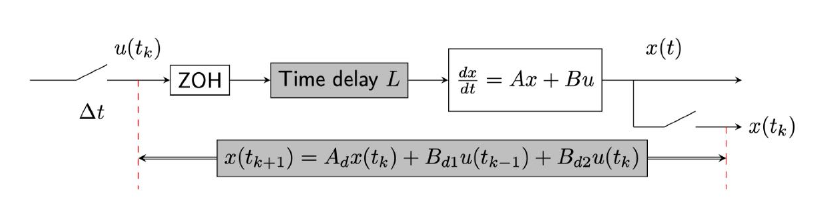
\includegraphics[width=0.7\textwidth]{ctrl_fig_7_3.png}

\section*{8 Stability}

\problem{8.1}{}
Show that the eigenvalues of skew-symmetric matrices are all imaginary or zero.

\problem{8.2}{}
Determine the range of $K$ so that the characteristic equation
\[
s^4 + 2.9s^3 + 0.7s^2 + 0.7s + (K - 0.1) = 0, \quad K > 0
\]
does not possess any root in the closed right-half complex plane.

\problem{8.3}{lyapunov-function-drills}
Consider the system $\dot{x} = -x + u$, where $x \in \mathbb{R}$ and $u \in \mathbb{R}$ is a control input. Show that the equilibrium point $x = 0$ is asymptotically stable using a Lyapunov function of the form $V(x) = \frac{1}{2}x^2$.

\problem{8.4}{lyapunov-function-drills}
Consider the system $\dot{x} = -x^3 + u$, where $x \in \mathbb{R}$ and $u \in \mathbb{R}$ is a control input. Show that the equilibrium point $x = 0$ is globally asymptotically stable using a Lyapunov function of the form $V(x) = \frac{1}{2}x^2$.

\problem{8.5}{lyapunov-function-drills}
Consider the system $\dot{x}_1 = -x_2$, $\dot{x}_2 = -x_1 + u$, where $x \in \mathbb{R}^2$ and $u \in \mathbb{R}$ is a control input. Show that the equilibrium point $x_1 = x_2 = 0$ is asymptotically stable using a Lyapunov function of the form $V(x) = \frac{1}{2}(x_1^2 + x_2^2)$.

\problem{8.6}{}
A continuous-time system is given by
\[
\frac{d}{dt}\begin{bmatrix} x_1(t) \\ x_2(t) \end{bmatrix} =
\begin{bmatrix} a & 1 \\ b & 0 \end{bmatrix}
\begin{bmatrix} x_1(t) \\ x_2(t) \end{bmatrix}.
\]
Based on the Lyapunov equation, show that $a$ and $b$ must be negative for asymptotic stability.

\problem{8.7}{}
Determine the stability of the discrete-time system
\[
x(k + 1) = \begin{bmatrix} 0 & 1 & 0 \\ 0 & 0 & 1 \\ 0.275 & -0.225 & -0.1 \end{bmatrix} x(k)
\]
by applying the Lyapunov equation in MATLAB or Python. The function \texttt{dlyap} might be useful for you.

\problem{8.8}{}
Consider an asymptotically stable second-order system
\[
\frac{d}{dt}\begin{bmatrix} x_1 \\ x_2 \end{bmatrix} =
\begin{bmatrix} 0 & 1 \\ -1 & -1 \end{bmatrix}
\begin{bmatrix} x_1 \\ x_2 \end{bmatrix}.
\]
Use the Lyapunov equation to find
\[
\int_0^{\infty} 2x_1^2(t) + qx_2^2(t)\,dt
\]
for $x_1(0) = 1$ and $x_2(0) = 0$.

\section*{9 Controllability and Observability}

\problem{9.1}{}
Consider the system $\dot{x} = Ax + Bu$, where $x \in \mathbb{R}^3$, $A = \begin{bmatrix} 1 & 2 & 3 \\ 4 & 5 & 6 \\ 7 & 8 & 9 \end{bmatrix}$ and $B = \begin{bmatrix} 1 \\ 0 \\ 1 \end{bmatrix}$. Determine whether the system is controllable or not.

\problem{9.2}{third-order-checks}
Consider a dynamic system with the following system matrices:
\[
A = \begin{bmatrix} -2 & 0 & 0 \\ 1 & 0 & 2 \\ 0 & 0 & 0 \end{bmatrix}, \quad
B = \begin{bmatrix} 1 \\ 0 \\ 1 \end{bmatrix}, \quad
C = \begin{bmatrix} 1 & 0 & 1 \end{bmatrix}.
\]
\begin{enumerate}
\item Show that the system is not observable by checking the rank of the observability matrix.
\item Now perform a similarity transform $\bar{x} = \begin{bmatrix} 1 & 0 & 0 \\ 0 & 0 & 1 \\ 0 & 1 & 0 \end{bmatrix} x$. Show that the third state in $\bar{x}$ is not observable.
\end{enumerate}

\problem{9.3}{}
Consider the following system with a diagonal $A$ matrix:
\[
\begin{aligned}
\frac{dx}{dt} &= \begin{bmatrix} \lambda_1 & 0 & 0 \\ 0 & \lambda_2 & 0 \\ 0 & 0 & \lambda_3 \end{bmatrix} x + \begin{bmatrix} b_1 \\ b_2 \\ b_3 \end{bmatrix} u, \\
y &= \begin{bmatrix} c_1 & c_2 & c_3 \end{bmatrix} x.
\end{aligned}
\]
Obtain conditions for controllability. Obtain conditions for observability.

\problem{9.4}{}
Consider a single-input, single-output third-order system described by
\[
\begin{aligned}
\frac{dx}{dt} &= \begin{bmatrix} a & 1 & 0 \\ b & 0 & 1 \\ c & 0 & 0 \end{bmatrix} x + \begin{bmatrix} 0 \\ d \\ 1 \end{bmatrix} u, \\
y &= \begin{bmatrix} e & 0 & 0 \end{bmatrix} x, \quad e > 0.
\end{aligned}
\]
Obtain the transfer function from $u$ to $y$. Examine the controllability and observability of this system. Show that a pole-zero cancellation in the transfer function takes place if this system is to lose either controllability or observability. Your answer to the last question should be based on the controllability matrix or the observability matrix. Recall that a square matrix is not full rank if and only if its determinant is zero.

\problem{9.5}{}
Consider a second-order discrete-time system described by
\[
\begin{bmatrix} x_1(k + 1) \\ x_2(k + 1) \end{bmatrix} =
\begin{bmatrix} \lambda_1 & 0 \\ 0 & \lambda_2 \end{bmatrix}
\begin{bmatrix} x_1(k) \\ x_2(k) \end{bmatrix} +
\begin{bmatrix} b_1 \\ b_2 \end{bmatrix} u(k), \quad 0 < \lambda_1 < 1, \quad 0 < \lambda_2 < 1.
\]
Obtain the controllability gramian, and find condition(s) for controllability based on the gramian.

\problem{9.6}{third-order-checks}
Consider a third-order system described by
\[
\begin{aligned}
\frac{dx}{dt} &= \begin{bmatrix} -2 & 0 & 0 \\ 1 & 0 & 1 \\ 0 & 0 & 0 \end{bmatrix} x + \begin{bmatrix} 1 \\ 0 \\ 1 \end{bmatrix} u, \\
y &= \begin{bmatrix} 1 & 0 & 1 \end{bmatrix} x.
\end{aligned}
\]
Is this system controllable? Is the system observable? Provide your analysis.

\problem{9.7}{}
Consider a discrete-time system described by
\[
\begin{aligned}
x_1(k + 1) &= x_2(k), \\
x_2(k + 1) &= -2x_1(k) - 3x_2(k) + u(k), \\
y(k) &= x_1(k) + x_2(k).
\end{aligned}
\]
Show that the system is not observable. Obtain all initial states which may not be distinguished from $\begin{bmatrix} x_1(0) & x_2(0) \end{bmatrix}^T = \begin{bmatrix} 1 & 0 \end{bmatrix}^T$ by the output measurement.

\problem{9.8}{}
The following system is known to be controllable:
\[
\dot{x} = Ax + Bu,
\]
where $x$ is an $n$-dimensional state vector and $u$ is an $m$-dimensional control input vector. Check whether the following systems are controllable:
\begin{enumerate}
\item $\dfrac{d}{dt}\begin{bmatrix} x_1 \\ x_2 \end{bmatrix} = \begin{bmatrix} A & 0 \\ 0 & A \end{bmatrix}\begin{bmatrix} x_1 \\ x_2 \end{bmatrix} + \begin{bmatrix} B \\ B \end{bmatrix} u$ where $\begin{bmatrix} x_1 \\ x_2 \end{bmatrix}$ is a $2n$-dimensional state vector.
\item $\dfrac{d}{dt}\begin{bmatrix} x_1 \\ x_2 \end{bmatrix} = \begin{bmatrix} A & 0 \\ 0 & A \end{bmatrix}\begin{bmatrix} x_1 \\ x_2 \end{bmatrix} + \begin{bmatrix} B & 0 \\ 0 & B \end{bmatrix}\begin{bmatrix} u_1 \\ u_2 \end{bmatrix}$ where $\begin{bmatrix} x_1 \\ x_2 \end{bmatrix} \in \mathbb{R}^{2n}$ and $\begin{bmatrix} u_1 \\ u_2 \end{bmatrix}$ is a $2m$-dimensional control input vector.
\end{enumerate}

\section*{10 Kalman Decomposition}

\problem{10.1}{}
A third-order system is described by
\[
\frac{dx}{dt} = \begin{bmatrix} -2 & 1 & 2 \\ 0 & 0 & 1 \\ 0 & 1 & 0 \end{bmatrix} x + \begin{bmatrix} 1 \\ 0 \\ 1 \end{bmatrix} u, \quad x(t_0) = x_0.
\]
\begin{enumerate}
\item Show, by hand calculation, that the system is uncontrollable but is stabilizable.
\item Use MATLAB to verify the conclusion in (a). Hint: from linear algebra, for a matrix $P \in \mathbb{R}^{n \times n}$, the $n$-dimensional vector space can be decomposed as $\mathbb{R}^n = \mathcal{R}(P) \oplus \mathcal{N}(P^T)$. Use the command \texttt{orth} to obtain an orthonormal basis for the range space of the controllability matrix $P$; use command \texttt{null(P')} to obtain the other vectors that complete the basis.
\end{enumerate}

\problem{10.2}{}
Consider the system $\dot{x} = Ax + Bu$, $y = Cx$, where $x \in \mathbb{R}^3$, $u \in \mathbb{R}$, $y \in \mathbb{R}$, $A = \begin{bmatrix} -1 & 0 & 1 \\ 0 & -2 & 0 \\ -1 & 0 & -1 \end{bmatrix}$, $B = \begin{bmatrix} 1 \\ 0 \\ 1 \end{bmatrix}$, $C = \begin{bmatrix} 1 & 0 & 0 \end{bmatrix}$. Find the Kalman decomposition of the system.

\section*{11 State Feedback}

\problem{11.1}{state-feedback-concepts}
Is controllability invariant under state feedback control? Why or why not?

\problem{11.2}{state-feedback-concepts}
Is controllability invariant under output feedback control? Why or why not?

\problem{11.3}{state-feedback-concepts}
What is the difference in terms of eigenvalue distributions between full-state feedback and output feedback control?

\problem{11.4}{pole-placement-drills}
Consider the following system:
\[
\dot{x} = \begin{bmatrix} 0 & 1 \\ -2 & -3 \end{bmatrix} x + \begin{bmatrix} 0 \\ 1 \end{bmatrix} u.
\]
Design a state feedback control law of the form $u = -Kx$ such that the closed-loop system has poles at $-1 \pm j$.

\problem{11.5}{pole-placement-drills}
Consider the following system:
\[
\dot{x} = \begin{bmatrix} 0 & 1 & 0 \\ 0 & 0 & 1 \\ -1 & -2 & -3 \end{bmatrix} x + \begin{bmatrix} 0 \\ 0 \\ 1 \end{bmatrix} u.
\]
Design a state feedback control law of the form $u = -Kx$ such that the closed-loop system has a settling time of less than 2 seconds and a percent overshoot of less than 10\%.

\section*{12 Observers and Observer-State Feedback}

\problem{12.1}{observer-concepts}
Can an observer be designed and effective if the system is unobservable? How and under what conditions?

\problem{12.2}{observer-concepts}
Is observability invariant under state-feedback control?

\problem{12.3}{}
What are the eigenvalues of the enlarged system in Example 12.5.1? Design your observer gain such that the eigenvalues are at $-1$, $-1$, $-1$, $-2$, and $-3$.

\problem{12.4}{}
A third-order system is described in observable canonical form:
\[
\begin{aligned}
\begin{bmatrix} x_1(k + 1) \\ x_2(k + 1) \\ x_3(k + 1) \end{bmatrix} &=
\begin{bmatrix} -a_2 & 1 & 0 \\ -a_1 & 0 & 1 \\ -a_0 & 0 & 0 \end{bmatrix}
\begin{bmatrix} x_1(k) \\ x_2(k) \\ x_3(k) \end{bmatrix} +
\begin{bmatrix} b_2 \\ b_1 \\ b_0 \end{bmatrix} u(k), \\
y(k) &= x_1(k).
\end{aligned}
\]
Design a discrete-time observer, which consists of the predictor and the corrector. Place all the observer eigenvalues at the origin. Show that when this observer is used, the estimation error is 0 at $k = 2$ for any initial state of the system at $k = 0$.

\problem{12.5}{}
Consider the discrete-time state-space equation
\[
\begin{aligned}
x(k + 1) &= \begin{bmatrix} 1 & 1 & -2 \\ 0 & 1 & 1 \\ 0 & 0 & 1 \end{bmatrix} x(k) + \begin{bmatrix} 1 \\ 0 \\ 1 \end{bmatrix} u(k), \\
y(k) &= \begin{bmatrix} 2 & 0 & 0 \end{bmatrix} x(k).
\end{aligned}
\]
Find the state feedback gain so that the resulting feedback system has all eigenvalues at $z = 0$. Show that for any initial state, the zero-input response of the feedback system becomes identically zero for $k \ge 3$.

\problem{12.6}{}
Consider a controllable and observable state-space model
\[
\frac{d}{dt}\underbrace{\begin{bmatrix} x_1 \\ x_2 \end{bmatrix}}_{\triangleq x} =
\underbrace{\begin{bmatrix} A_{11} & 0 \\ A_{21} & A_{22} \end{bmatrix}}_{\triangleq A}
\begin{bmatrix} x_1 \\ x_2 \end{bmatrix} +
\underbrace{\begin{bmatrix} B_1 \\ B_2 \end{bmatrix}}_{\triangleq B} u, \quad
y = \underbrace{\begin{bmatrix} I_s & 0 \\ 0 & C_2 \end{bmatrix}}_{\triangleq C}
\begin{bmatrix} x_1 \\ x_2 \end{bmatrix},
\]
where $x_1 \in \mathbb{R}^{s \times 1}$, $x_2 \in \mathbb{R}^{(n-s) \times 1}$, $u \in \mathbb{R}^{m \times 1}$, $y \in \mathbb{R}^{(s+1) \times 1}$, and $x_1$ is directly measurable. Suppose a full state observer is used:
\[
\dot{\widehat{x}} = A\widehat{x} + Bu + L\left(y - C\widehat{x}\right).
\]
In the state feedback law, the measurable state, $x_1$, is directly used, i.e., $u = -K\begin{bmatrix} x_1^T & \widehat{x}_2^T \end{bmatrix}$. Notice that the control law is a mixture of state feedback control and observer state feedback control, and that the order of the overall system is $2n$. Show that $n$ closed-loop eigenvalues satisfy $\det[\lambda I_n - (A - BK)] = 0$, and other $n$ closed eigenvalues satisfy $\det[\lambda I_n - (A - LC)] = 0$.

\problem{12.7}{}
Given the following system
\[
\begin{aligned}
\dot{x} &= Ax + Bu + Bd, \quad A \in \mathbb{R}^{n \times n}, \\
y &= Cx,
\end{aligned}
\]
where $d$ is a disturbance that satisfies the model
\[
\dot{d} = A_d d, \quad A_d \in \mathbb{R}^{n_d \times n_d}.
\]
Assume that $(A, B)$ is controllable and $(A, C)$ is observable.
\begin{enumerate}
\item Augment the system so that the augmented state is $\bar{x} = \begin{bmatrix} x \\ d \end{bmatrix}$.
\item Design a Luenberger observer for the augmented system you derived in part a.
\item Assume that $A$ is nonsingular and $A_d = 0$, i.e., $d$ is a constant unknown disturbance. Derive the observability condition for the augmented system.
\item Derive the general observability condition when $A_d \in \mathbb{R}^{n_d \times n_d}$.
\item Analyze the error dynamics and eigenvalues of the observer for the augmented system.
\end{enumerate}

\problem{12.8}{}
Recode Example 12.2.1 using Simulink. This time, use a separate Simulink block for the plant and a separate block for the observer.

\section*{13 Linear Quadratic Optimal Control}

\problem{13.1}{lq-concepts}
What is the goal of linear quadratic optimal control?

\problem{13.2}{lq-concepts}
How is the optimal control law derived in linear quadratic optimal control?

\problem{13.3}{lq-concepts}
What is the role of the weighting matrices $Q$ and $R$ in the cost function of linear quadratic optimal control? How does the choice of the weighting matrices affect the performance of the control system?

\problem{13.4}{lq-concepts}
Explain the difference between state feedback control and output feedback control.

\problem{13.5}{lq-concepts}
What is the importance of system observability and controllability in the design of optimal control systems?

\problem{13.6}{lq-concepts}
Explain the trade-off between control effort and performance in linear quadratic optimal control.

\problem{13.7}{lq-concepts}
What is Bellman's Principle of Optimality?

\problem{13.8}{}
Consider a two-mass two-spring system below
\[
\frac{d}{dt}\begin{bmatrix} v_{m_1} \\ v_{m_2} \\ f_{k_1} \\ f_{k_2} \end{bmatrix} =
\begin{bmatrix}
0 & 0 & -\frac{1}{m_1} & \frac{1}{m_2} \\
0 & 0 & 0 & -\frac{1}{m_2} \\
k_1 & 0 & 0 & 0 \\
-k_2 & k_2 & 0 & 0
\end{bmatrix}
\underbrace{\begin{bmatrix} v_{m_1} \\ v_{m_2} \\ f_{k_1} \\ f_{k_2} \end{bmatrix}}_{x} +
\begin{bmatrix} 0 \\ \frac{1}{m_2} \\ 0 \\ 0 \end{bmatrix} u.
\]
Assume $m_1 = m_2 = 1$ and $k_1 = k_2 = 1$.
\begin{enumerate}
\item Show that the transfer function from $u$ to $v_{m_2}$ is given by
\[
\frac{V_{m_2}(s)}{U(s)} = \frac{s\left(s^2 + 2\right)}{s^4 + 3s^2 + 1}.
\]
\item For this system, an optimal LQ problem is formulated with the quadratic performance index
\[
J = \int_0^{\infty} \left[x_{m_2}^2(t) + Ru^2(t)\right] dt,
\]
where $x_{m_2} = \begin{bmatrix} 0 & 0 & 1 & 1 \end{bmatrix} x$. Obtain the optimal feedback control gain for $R = 0.0001$, $1$ and $1{,}000$. For each $R$, use MATLAB or Python to obtain the response of the optimal closed loop system for $f_{k_1}(0) = 1$. The initial conditions of other state variables are zero.
\end{enumerate}

\problem{13.9}{}
Consider a third-order system described by
\[
\frac{d}{dt}\begin{bmatrix} x_1 \\ x_2 \\ x_3 \end{bmatrix} =
\begin{bmatrix} 0 & 1 & 0 \\ 0 & 0 & 1 \\ 0 & 0 & 0 \end{bmatrix}
\begin{bmatrix} x_1 \\ x_2 \\ x_3 \end{bmatrix} +
\begin{bmatrix} 0 \\ 0 \\ 1 \end{bmatrix} u.
\]
The control input is to be determined to minimize the performance index
\[
J = \int_0^{\infty} \left\{x_1^2 + 2x_2^2 + x_3^2 + Ru^2\right\} dt. \tag{13.98}
\]
\begin{enumerate}
\item Draw the symmetric root locus.
\item Obtain the value of $R$ when the optimal system has a pair of complex eigenvalues, $\lambda_{1,2} = -\sigma \pm j\sigma$ ($\sigma > 0$). What is the third eigenvalue of the optimal system in this case?
\item Draw the symmetric root locus for the performance index
\[
J = \int_0^{\infty} \left\{x_1^2 + 2x_1x_2 + 2x_2^2 + x_3^2 + Ru^2\right\} dt. \tag{13.99}
\]
Show that the symmetric root locus for Equation 13.98 and that for Equation 13.99 are the same. Actually, in this problem, the cross product term $2x_1x_2$ does not influence the optimal control law. Show that this is true by evaluating
\[
\int_0^{\infty} x_1x_2\,dt.
\]
Note that the closed loop system is asymptotically stable since the controllability and observability assumptions are satisfied.
\item Let $R = 0.1$, $1$, and $10000$. For the performance index Equation 13.98, use MATLAB to obtain the Nyquist plot of the optimal loop transfer function in Section 13.5.2 to check that the gain margin and phase margin conditions are satisfied. You need to explicitly mention how you treat the three open-loop poles at the origin, i.e. treat them as poles in the left half side or the right half side of the s-plane, to conclude the nominal stability.
\end{enumerate}

\problem{13.10}{}
How do you split one number, say $x_f$, to $N$ pieces so that the product of the $N$ pieces is maximized? Think in the following way. We have an integrator described by
\[
x(k + 1) = x(k) + u(k), \quad x(0) = 0, \quad x(N) = x_f,
\]
where $u(k) \ge 0$. Our goal is then to find $\{u(0), u(1), \dots, u(N - 1)\}$ so that
\[
J = \prod_{i=0}^{N-1} u(i) = u(0)u(1) \cdots u(N - 1)
\]
is maximized. You can solve this problem by applying dynamic programming. For this purpose, define
\[
J_k(x(k)) = \prod_{i=k}^{N-1} u(i).
\]
Start by showing that $J_{N-1}^0(x(N - 1)) = x_f - x(N - 1)$.

\problem{13.11}{}
In this problem, we extend the analysis on the pendulum system in Section 13.4.4.
\begin{enumerate}
\item Change the code to plot also the control action $u$. Change the weighting $R$ and see the effects on the resulting optimal control $u$.
\item Add a step change of the cart position at 6 second of the simulation. Tune the controller and evaluate the performance.
\item Rewrite the simulations using MATLAB.
\item In Section 13.4.4, we applied LQ and the state observer to the linearized plant. Implement the observer state feedback on the nonlinear system model instead. Plot the estimated states plus the equilibrium point, and compare them with the actual states of the nonlinear system.
\end{enumerate}

\section*{14 Review of Probability Theory}

\problem{14.1}{random-process-concepts}
What is the difference between a discrete and a continuous random process? Give an example of each and explain how to characterize them mathematically.

\problem{14.2}{random-process-concepts}
What is the autocorrelation function of a random process? How does it relate to the power spectral density? How can you estimate them from a finite sample of data?

\problem{14.3}{random-process-concepts}
What is the ergodicity property of a random process? How can you test if a random process is ergodic or not? What are the implications of ergodicity for statistical inference?

\problem{14.4}{random-process-concepts}
What is the difference between a stationary and a non-stationary random process? Give an example of each and explain how to model them using linear filters or state-space models.

\problem{14.5}{random-process-concepts}
What are some applications of random processes in engineering, science, or everyday life? How can you use random processes to model uncertainty, noise, or variability in these domains?

\problem{14.6}{}
The sum of $N$ independent random variables with uniform distributions approaches a Gaussian random variable as $N \to \infty$. Consider three independent random variables, $x_1$, $x_2$ and $x_3$. Each of them is uniformly distributed between 0 and 1. Obtain the probability density function for $x_1 + x_2$ and $x_1 + x_2 + x_3$. HINT: Let $z = x_1 + x_2$. Then, $z$ and $x_1$ are dependent, and $p_z(z|x_1) = p_{x_2}(z - x_1)$. Furthermore,
\[
\begin{aligned}
p_z(z) &= \int_{-\infty}^{\infty} p(z, x_1)dx_1 = \int_{-\infty}^{\infty} p_z(z|x_1)p_{x_1}(x_1)dx_1 \\
&= \int_{-\infty}^{\infty} p_{x_2}(z - x_1)p_{x_1}(x_1)dx_1.
\end{aligned}
\]

\problem{14.7}{}
For a random vector $x$, the covariance matrix $X$ is defined by
\[
X = E[(x - m_x)(x - m_x)^T],
\]
where $m_x = E[x]$. Notice that the matrix, $(x - m_x)(x - m_x)^T$, cannot be positive definite. Show $X$ is at least positive semidefinite and that $X$ is positive definite if the variance of $\alpha^T(x - m_x)$ is positive for any deterministic vector $\alpha$.

\problem{14.8}{}
Determine the autocovariance (autocorrelation) function $X_{yy}(k)$ and the spectral density $\Phi_{yy}(\omega)$, of the process $y(k)$ when
\[
y(k) - 0.8y(k - 1) = e(k) + 0.5e(k - 1),
\]
where $e(k)$ is a zero mean white random signal with unit variance.

\problem{14.9}{}
A continuous-time system is given by
\[
\begin{aligned}
\frac{d}{dt}\begin{bmatrix} x_1 \\ x_2 \end{bmatrix} &=
\begin{bmatrix} 0 & 1 \\ -2 & -3 \end{bmatrix}
\begin{bmatrix} x_1 \\ x_2 \end{bmatrix} +
\begin{bmatrix} 0 \\ 1 \end{bmatrix} w(t), \\
y(t) &= \begin{bmatrix} 1 & 0.5 \end{bmatrix} \begin{bmatrix} x_1 \\ x_2 \end{bmatrix},
\end{aligned}
\]
where $x(0) = 0$ and $w(t)$ is a white zero mean random process with $E[w^2(t)] = 1$. Obtain the variance, auto-correlation and spectral density of $y(t)$ at the steady state.

\section*{15 Least Square Estimation}

\problem{15.1}{}
Explain what is the goal of least square estimation and what are the assumptions behind it.

\problem{15.2}{}
Consider a (first-order) discrete-time system described by
\[
x(k + 1) = ax(k) + w(k) + c,
\]
where $x(0)$ and $c$ are random variables, and $w(k)$ is a white random process (sequence) with $E[x(0)] = 0$, $E[x^2(0)] = 4$, $E[w(k)] = 0$, $E[w(k)w(j)] = W\delta_{kj}$, $E[c] = 0$, $E[c^2] = C$, $E[x(0)c] = 0$, $E[x(0)w(k)] = 0$, $E[w(k)c] = 0$. $c$ remains constant once an experiment starts.
\begin{enumerate}
\item Write equations for computing the variance of $x(k)$. Do not forget to give the initial condition for the equations. You do not have to solve the equations.
\item Assume that the system is asymptotically stable. Obtain the variance of $x(k)$ at the steady state.
\end{enumerate}

\section*{16 Stochastic State Estimation and Kalman Filter}

\problem{16.1}{}
Derive the Kalman-filter gain formula for a discrete-time system with additive Gaussian noise. Show how the Kalman filter minimizes the mean squared error of the state estimate.

\problem{16.2}{}
A constant value $x$ is repeatedly measured. The measurement process involves noise effects. Assume that the system is described by
\[
y(k) = x + v(k)
\]
where $y(k)$ is the $k$-th measurement, $v(k)$ is the measurement noise, and $x$ and $v(k)$ are Gaussian distributed with $E[x] = 0$, $E[x^2] = X_0$, $E[v(k)] = 0$, $E[v(k)v(j)] = V\delta_{kj}$, $E[x(0)v(k)] = 0$.
\begin{enumerate}
\item Obtain the least square estimate
\[
\widehat{x}(k) = E[x \mid y(0), y(1), \dots, y(k)]
\]
and the estimation error covariance.
\item Show that in the limit of $X_0$ approaching to $\infty$, i.e., no prior information on $x$, $\widehat{x}(k)$ and the estimation error covariance, respectively, are asymptotic to $[y(0) + y(1) + \dots + y(k)]/(k + 1)$ and $V/(k + 1)$. Solve this problem in two ways. In the first approach, regard that $y(0)$, $y(1)$, $y(2)$, etc as elements of a random vector $Y_{vec}$: i.e.
\[
Y_{vec} = [y(0), y(1), \dots, y(k)]^T
\]
and apply the least square formula once. In this case, check part b for $k = 2$. In the second approach, you consider the measurement equation along with the state equation, $x(k + 1) = x(k)$, and apply the Kalman filter equations to the problem.
\end{enumerate}

\problem{16.3}{}
Implement a simple Kalman filter in Python for a one-dimensional constant velocity model. Use simulated measurements with noise and plot the true state, the measurements and the filtered state over time.

\problem{16.4}{}
Derive the return difference equality for the steady-state continuous-time Kalman filter.

\problem{16.5}{}
Consider Example 16.2.1 about the discrete-time Kalman filter for a second-order system. Use MATLAB and Python to work on the following.
\begin{enumerate}
\item Obtain the steady-state Kalman-filter gain and estimation-error covariance matrix for $r = 0.05$ and $6$. Compare the results from MATLAB and Python. Try decrease $r$ further and identify the root cause of the numerical issue in Python.
\item Simulate the time response of the system and the Kalman filter for the above values of $r$. Observe whether the results are to your expectation.
\item Utilize the return difference equality and draw a root locus plot for $r$ varying from 0 to $\infty$.
\item Show that $e_y(k)$ is a white random sequence.
\end{enumerate}

\section*{17 Linear Quadratic Gaussian (LQG) Optimal Control}

\problem{17.1}{lqg-concepts}
What is the separation principle of LQG control and why is it useful?

\problem{17.2}{lqg-concepts}
What are the advantages and disadvantages of LQG control compared to other optimal control methods?

\problem{17.3}{lqg-concepts}
How does LQG control handle disturbances and measurement noise in a linear system?

\problem{17.4}{lqg-concepts}
What are the conditions for the stability and robustness of the closed-loop system under LQG control?

\problem{17.5}{}
A discrete-time system is described by
\[
x(k + 1) = Ax(k) + Bu(k) + B_w w(k),
\]
where $w(k)$ is a colored noise given by
\[
\begin{aligned}
w(k) &= C_w x_w(k), \\
x_w(k + 1) &= A_w x_w(k) + B_n n(k).
\end{aligned}
\]
$x(0)$, $x_w(0)$ and $n(k)$ are independent and Gaussian distributed with
\[
\begin{aligned}
E[x(0)] &= x_0, & E\left[(x(0) - x_0)(x(0) - x_0)^T\right] &= X_0, \\
E[x_w(0)] &= x_{w0}, & E\left[(x_w(0) - x_{w0})(x_w(0) - x_{w0})^T\right] &= X_{w0}, \\
E[n(k)] &= 0, & E\left[n(k)n^T(k)\right] &= N\delta_{kj}.
\end{aligned}
\]
The performance index to be minimized is
\[
J = E\left[x^T(N)Sx(N) + \sum_{j=0}^{N-1} \left\{x^T(j)Qx(j) + u^T(j)Ru(j)\right\}\right]
\]
where the expectation must be taken over all underlying random quantities in each of the following three situations. Consider the following three cases, and obtain equations to find the optimal control for each case.
\begin{enumerate}
\item $x(k)$ and $x_w(k)$ are directly accessible.
\item $y(k) = Cx(k) + v(k)$ is the only measurement where $v(k)$ is a zero mean, white, Gaussian noise with $E[v(k)v^T(j)] = V\delta_{kj}$, and is independent from $x(0)$, $x_w(0)$ and $n(k)$.
\item $x(k)$ is directly accessible. For this part of the problem, notice that
\[
x(k) - Ax(k - 1) - Bu(k - 1) = B_w C_w x_w(k - 1).
\]
This means that at time $k$, the measurement, or the directly accessible data, reflects information only about the random vector $x_w(k - 1)$ (i.e. there is a one-step delay). Also, when considering
\[
x(k) - Ax(k - 1) - Bu(k - 1) = B_w C_w x_w(k - 1),
\]
we can regard that there is no measurement noise for the state $x_w(k - 1)$. Therefore, if you set the measurement covariance matrix to 0 and find a Kalman filter for estimating $x_w$, you obtain
\[
\widehat{x}_w(k - 1 \mid k) = \widehat{x}_w(k - 1 \mid x(0), x(1), \dots, x(k)).
\]
\end{enumerate}

\problem{17.6}{}
Consider a second-order system described by
\[
\begin{aligned}
\frac{d}{dt}\begin{bmatrix} x_1(t) \\ x_2(t) \end{bmatrix} &=
\begin{bmatrix} 1 & 1 \\ 0 & 1 \end{bmatrix}
\begin{bmatrix} x_1(t) \\ x_2(t) \end{bmatrix} +
\begin{bmatrix} 0 \\ b \end{bmatrix} u(t) +
\begin{bmatrix} 1 \\ 1 \end{bmatrix} w(t), \\
y(t) &= \begin{bmatrix} 1 & 0 \end{bmatrix} \begin{bmatrix} x_1(t) \\ x_2(t) \end{bmatrix} + v(t),
\end{aligned}
\]
where $w(t)$ and $v(t)$ are zero mean, white Gaussian random processes with $E[w(t)w(t + \tau)] = W\delta(\tau)$ and $E[v(t)v(t + \tau)] = V\delta(\tau)$. The initial state is a Gaussian random vector. $x(0)$, $w(t)$ and $v(t)$ are independent. Suppose that we know the nominal value of $b$ is 1 but we do not know $b$ exactly. The performance index is
\[
J = E\left[x^T(t)Qx(t) + \rho u^2(t)\right], \quad \rho > 0, \quad
Q = \begin{bmatrix} 1 \\ 1 \end{bmatrix}\begin{bmatrix} 1 & 1 \end{bmatrix}.
\]
This is a stationary LQG problem.
\begin{enumerate}
\item Assume that the state vector is exactly known (i.e. directly measurable). Assume that $b = 1$, and obtain the optimal control (you can obtain it analytically). The LQ control feedback gain will be in the form of $\alpha[1, 1]$.
\item Calculate the closed-loop eigenvalues for $\rho = 0.2$ and $b = 1$. Verify that the system is stable for $0.5 < b \le \infty$. (Assume that the state vector is exactly known.)
\item Let $W = 1$ and $V = \sigma$. Obtain the Kalman filter gain analytically (assume $b = 1$). The Kalman filter gain will be in the form $\beta\begin{bmatrix} 1 \\ 1 \end{bmatrix}$. Note that if the LQ and KF gains are obtained for the nominal value of $b$ (i.e. $b = 1$), the closed-loop eigenvalues of the actual system are the eigenvalues of the matrix
\[
\bar{A}_c = \begin{bmatrix}
1 & 1 & 0 & 0 \\
0 & 1 & -b\alpha & -b\alpha \\
\beta & 0 & 1 - \beta & 1 \\
\beta & 0 & -\beta - \alpha & 1 - \alpha
\end{bmatrix}.
\]
\item Let $\rho = 0.2$ and $\sigma = 5$ and $b = 1$. Calculate the eigenvalues of $\bar{A}_c$ and confirm the separation theorem for eigenvalues.
\item Let $\rho = 0.2$ and $\sigma = 5$ and $b = 1.1$. What do you think of the stability of the LQG system? Calculate the eigenvalues of the closed-loop $A$ matrix to confirm your guess. (A message from this part: the excellent robustness properties of the LQ control system will no longer hold in state estimator feedback control.)
\end{enumerate}

\end{document}
